\documentclass[11pt]{article}
\usepackage[a4paper,margin=25mm]{geometry}
\usepackage[T1]{fontenc}
\usepackage[utf8]{inputenc}
\usepackage{lmodern,microtype}
\usepackage{amsmath,amssymb,amsthm,mathtools}
\usepackage{booktabs,array,graphicx,xcolor,enumitem}
\usepackage{flafter}
\usepackage[section]{placeins}
\usepackage[hidelinks]{hyperref}
\hypersetup{pdftitle={Two clocks for quantum information},
 pdfauthor={Research construction note},
 pdfsubject={Finite action law and output-only recovery through mixed collision baths}}
\usepackage{url}
\setlist{itemsep=3pt,topsep=5pt}
\setlength{\emergencystretch}{2em}
\numberwithin{equation}{section}
\newtheorem{theorem}{Theorem}[section]
\newtheorem{lemma}[theorem]{Lemma}
\newtheorem{corollary}[theorem]{Corollary}
\newtheorem{proposition}[theorem]{Proposition}
\theoremstyle{remark}
\newtheorem{remark}[theorem]{Remark}
\newcommand{\Tr}{\operatorname{Tr}}
\newcommand{\id}{\operatorname{id}}
\newcommand{\Ad}{\operatorname{Ad}}
\newcommand{\supp}{\operatorname{supp}}
\newcommand{\rank}{\operatorname{rank}}
\newcommand{\Ccal}{\mathcal C}
\newcommand{\Dcal}{\mathcal D}
\newcommand{\Rcal}{\mathcal R}
\newcommand{\Pcal}{\mathcal P}
\newcommand{\Qcal}{\mathcal Q}
\newcommand{\Ucal}{\mathcal U}
\newcommand{\norm}[1]{\left\lVert#1\right\rVert}
\newcommand{\ip}[2]{\left\langle#1,#2\right\rangle}
\newcommand{\ket}[1]{\lvert#1\rangle}
\newcommand{\bra}[1]{\langle#1\rvert}
\newcommand{\dd}{\,\mathrm d}
\newcommand{\eps}{\varepsilon}
\title{Two clocks for quantum information:\\
 a finite action law for acquisition through mixed collision baths}
\author{Research construction note}
\date{5 November 2026}
\begin{document}
\maketitle

\begin{abstract}
The rate at which an open quantum system forgets its state does not determine
the rate at which its physically accessible mixed environment acquires that
state. We resolve this distinction for a finite collision interface. A finite
source interacts once with each fresh maximally mixed register; initial
purifiers and the final source are unavailable to the receiver. The receiver
may retain all emitted correlations, perform arbitrary quantum instruments,
and send classical feedback selecting later interactions. If round \(j\) has
interaction action at most \(a_j\) on every branch, the entire acquired channel
is close to a replacer when \(\sum_j a_j^4\) is small. Accurate recovery
requires \(\sum_j a_j^4=\Omega(\log(1/\eps))\) under uniformly weak collisions.
For partial SWAP, a mixed dummy and reversed collision circuit give an exact
recovered channel with residual \(\prod_j(1-\sin^4\theta_j)\). Established
transpose-recovery inequalities put this receiver within a factor two of
every decoder's worst-case channel error. The source forgets on the faster
\(\prod_j\cos^2\theta_j\) clock. We specify finite timing, memory, preparation,
calibration, and error costs, and separate dense small-system checks from
large-resource formula evaluations. The interface is a physical premise; it
is not inferred from a reduced generator.
\end{abstract}

\section{Question, outcome, and selection}
\label{sec:question}
An arbitrary unknown quantum state is held by a source that repeatedly meets
fresh bath registers. A receiver obtains every emitted physical register,
with chronological labels and complete coherent access. When can it recover
the input after the source itself has become unavailable?

This differs from reversing the whole closed system and from receiving the
complete complementary channel of a pure Stinespring dilation. A mixed bath
can have an inaccessible purification. Observing source relaxation does not
add that purifier to the receiver's resources.

We answer the question for fresh \emph{tracial} registers: each starts
maximally mixed. The principal result is a finite action law including all
emitted correlations and genuine classical feedback. An exact partial-SWAP
construction attains its weak-collision order. Petz recovery and its
near-optimality are established machinery; the acquisition bound and the
exact physical clock are the substantive calculation.

Throughout, channel error means \emph{half} the diamond distance,
\begin{equation}
 d_\diamond(\Lambda,\Gamma):=\tfrac12\norm{\Lambda-\Gamma}_{\diamond}.
 \label{eq:convention}
\end{equation}
Thus \(0\le d_\diamond\le1\) for channels. Recovery guarantees cover every
reference entangled with the unknown input.

\paragraph{Independent construction before selection.}
Several different questions were developed before selection. A computational
construction connected local unit-rate dynamics to long non-normal
transients and succinct prediction hardness; its consequence overlapped
established obstructions and required an unprovided persistent-error
compiler. A nonquantum construction proved an exact ambiguity in internal
dissipation under feedback through specified force/position ports, even with
a known observable and controllable drift. Its completed consequence was an
identification obstruction. A separate pure-port weak-export route stopped
at a gap between source/reference decoupling and an efficient decoder.
The present route supplies both a general
limitation and an operation attaining its scale. Companion selection notes
retain the independent constructions. Earlier Astra results are premises
and comparators, not objects of a new validation campaign.

\paragraph{Supplied access.}
The model supplies a finite source, fresh independent maximally mixed inputs,
known coupling reach, no return path, and unavailable purifiers. The
constructive receiver also needs coherent retention. These facts are not
inferred from short observations. Section~\ref{sec:physical} exposes their
costs. A strong source SWAP, when available, remains a one-collision export.

\section{Interface and universal statement}
\label{sec:interface}
The source \(S\) has fixed finite dimension \(d\ge2\). Round \(j\) introduces
a finite register \(E_j\) in \(I_{E_j}/e_j\), independent of the source,
reference, receiver, and other fresh registers. Its purifier is inaccessible.
After one collision the receiver obtains \(E_j\); it never returns to the
source. The source is discarded after at most \(N\) rounds.

The receiver has arbitrary finite quantum memory initialized independently of
the input. Between rounds it may apply arbitrary instruments, retain every
outcome, and use a \emph{dephased classical history} \(h\) to select later
collision Hamiltonians and source-only unitary controls. It retains arbitrary
coherent output correlations. Retained quantum memory never couples coherently
to \(S\), and there is no source measurement/reset or extra source port.
Bounded stopping is included by zero-action padding. All spaces and record
sets are finite, without a bound on their size.

Set \(\hbar=1\). After removing source-only and fresh-register-only controls
in an interaction picture, suppose
\begin{equation}
 a_{j,h}:=\int_{\text{round }j}
       \norm{H_{j,h}(t)}_\infty\dd t\le a_j
       \quad\text{for every classical history }h.
 \label{eq:action}
\end{equation}
The action is integrated over the \emph{entire encounter with one fresh
register}. Subdividing that encounter into time slices does not create
fresh collisions or reduce its charged action.
The history is fixed during each collision. These are deterministic
branchwise integrated bounds, not bounds on average action. Let \(\Ccal_N\)
be the channel to all retained outputs and records, and put
\begin{equation}
 \sigma_N:=\Ccal_N(I/d),\qquad
 \Rcal_{\sigma_N}(X):=\Tr(X)\sigma_N.
\end{equation}
Define
\begin{equation}
 q_j:=\min\{1,4a_j^4\},\quad
 b_N:=\prod_j(1-q_j),\quad
 \alpha_N:=1-b_N,\quad c_d:=1-d^{-2}.
 \label{eq:parameters}
\end{equation}

\begin{theorem}[Adaptive tracial acquisition law]
\label{thm:universal}
The stated interface obeys
\begin{align}
 d_\diamond(\Ccal_N,\Rcal_{\sigma_N})
  &\le\min\left\{1,\tfrac12\sqrt{(d^2-1)\alpha_N}\right\},
       \label{eq:universal-output}\\
 \inf_{\mathcal R}d_\diamond(\mathcal R\Ccal_N,\id)
  &\ge c_d(1-\sqrt{\alpha_N})\ge\tfrac{c_d}{2}b_N.
       \label{eq:universal-recovery}
\end{align}
The infimum includes every CPTP decoder on the entire receiver output,
without computational, memory, or ancillary-resource restrictions.
\end{theorem}

\begin{corollary}[Action required for accurate recovery]
\label{cor:action}
If \(4a_j^4\le q_*<1\) for all \(j\), then
\begin{equation}
 \inf_{\mathcal R}d_\diamond(\mathcal R\Ccal_N,\id)
 \ge\frac{c_d}{2}
 \exp\left[-\frac{4\sum_j a_j^4}{1-q_*}\right].
 \label{eq:action-converse}
\end{equation}
Achieving \(0<\eps<c_d/2\) requires
\begin{equation}
 \sum_j a_j^4\ge\frac{1-q_*}{4}\log\frac{c_d}{2\eps}.
 \label{eq:action-budget}
\end{equation}
\end{corollary}
\begin{proof}
Apply \(\log(1-q)\ge-q/(1-q_*)\) to the product in
\eqref{eq:universal-recovery}.
\end{proof}

The constants depend on source dimension, not total bath dimension. The
conclusion changes with nontracial fresh inputs, accessible preparation
labels or purifiers, returned registers, coherent feedback, or extra source
access. Strong collisions are allowed, but \(q_j=1\) makes this bound
uninformative. Section~\ref{sec:pathwise} permits history-dependent budgets.

\section{Proof of the adaptive acquisition law}
\label{sec:proof}
\subsection{A contracting weighted operator norm}
For a positive baseline \(\omega\), on its support define
\begin{equation}
 \norm{X}_\omega^2:=\Tr(X^\dagger X\omega^{-1}).
 \label{eq:weighted}
\end{equation}
Inverses are support inverses; the weight need not have unit trace.

\begin{lemma}[Data processing and source projection]
\label{lem:weighted}
Every CPTP map \(\Phi\) satisfies
\begin{equation}
 \norm{\Phi(X)}_{\Phi(\omega)}\le\norm{X}_{\omega}.
 \label{eq:weighted-contract}
\end{equation}
Appending a fixed state is an isometry, as is conjugation by a unitary
commuting with \(\omega\). If \(\Tr\omega=1\), then
\(\norm{X}_1\le\norm{X}_{\omega}\).
For \(\omega=I_S/d\otimes\sigma_M\), the map
\begin{equation}
 \Pcal X=I_S/d\otimes\Tr_SX,\qquad \Qcal=I-\Pcal
 \label{eq:projection}
\end{equation}
is an orthogonal projection in this norm, and
\begin{equation}
 \norm{\Pcal X}_{\omega}^2=\norm{\Tr_SX}_{\sigma_M}^2.
 \label{eq:projection-norm}
\end{equation}
Receiver-only maps commute with both projections and contract their norms
separately.
\end{lemma}
\begin{proof}
The variational formula
\[
 \norm{X}_{\omega}^2
 =\sup_Y\{2\operatorname{Re}\Tr X^\dagger Y
                 -\Tr\omega Y^\dagger Y\}
\]
and the Schwarz inequality for the unital CP adjoint \(\Phi^\dagger\) prove
\eqref{eq:weighted-contract}. Pull an output test \(Y\) back and use
\(\Phi^\dagger(Y^\dagger Y)\ge
\Phi^\dagger(Y)^\dagger\Phi^\dagger(Y)\).
Restriction to supports or regularization handles singular baselines.
The isometries follow by substitution. The trace-norm bound follows from
Hilbert--Schmidt H\"older applied to
\((X\omega^{-1/2})\omega^{1/2}\).
If \(\Tr_SZ=0\), its weighted inner product with \(I/d\otimes A\) is zero.
This proves orthogonality; substitution proves \eqref{eq:projection-norm}.
Receiver maps commute with the source trace, proving the last assertion.
\end{proof}

\subsection{The reference process stays product}
Run the same protocol with source input \(I/d\). At every stage the joint
baseline is
\begin{equation}
 \omega=I_S/d\otimes\sigma_M .
 \label{eq:baseline}
\end{equation}
In each classical history block, the fresh source/register factor is
\(I_S/d\otimes I_{E_j}/e_j\), invariant under the selected unitary. Receiver
maps change only \(\sigma_M\), and source-only unitaries preserve \(I/d\).
This proves \eqref{eq:baseline} inductively. A spectator reference may be
included in \(M\), with factor \(\rho_R\) in the baseline.

The selected Hamiltonian commutes with the baseline within each classical
block. This is the point at which genuine classical control matters. The
same statement does not hold for a coherent control register entangled with
the source or for a coupling to retained quantum receiver memory.

\subsection{One collision exports only second-order amplitude}
\begin{lemma}[Fresh tracial transfer]
\label{lem:onecollision}
For one history block with action \(a\), append \(I_E/e\) and let
\(y=\norm{\Pcal X}_\omega^2\), \(z=\norm{\Qcal X}_\omega^2\).
The collision changes these to
\begin{equation}
 y'=y+t,\qquad z'=z-t,\qquad
 0\le t\le\min\{1,4a^4\}\,z .
 \label{eq:collision-recursion}
\end{equation}
\end{lemma}
\begin{proof}
The old \(\Pcal X\otimes I_E/e\) commutes with the unitary and is unchanged.
For every Hamiltonian on \(SE\),
\begin{equation}
 \Pcal[H,\Qcal X\otimes I_E/e]=0.
 \label{eq:first-order-zero}
\end{equation}
Expand \(H\) in source and fresh-register matrices and \(\Qcal X\) in source
and old-memory matrices. Each partial source trace is the trace of a
commutator, hence zero. Exact traciality and the stated coupling reach are
both used here.

Write \(\mathcal L_t=-i[H(t),\,\cdot\,]\) and
\(\Ucal_t=\Ad_{U_t}\). The exact Volterra identity is
\[
 \Ucal_T=I+\int_0^T\mathcal L_s\dd s+
     \int_{0\le r\le s\le T}\mathcal L_s\mathcal L_r\Ucal_r
                  \dd r\dd s .
\]
The propagators are weighted-norm isometries and
\(\norm{\mathcal L_t Z}_\omega\le
2\norm{H(t)}_\infty\norm Z_\omega\).
Apply \(\Pcal\) to input \(\Qcal X\otimes I_E/e\).
Its zeroth and first terms vanish. The remainder has norm at most
\(2a^2\norm{\Qcal X}_\omega\). Projection and unitarity also bound it by
\(\norm{\Qcal X}_\omega\), proving the bound on \(t\).
The transfer is orthogonal to the old \(\Pcal\) component:
\[
 \ip{\Pcal X}{\Pcal\Ad_U\Qcal X}_\omega
 =\ip{\Ad_{U^{-1}}\Pcal X}{\Qcal X}_\omega=0,
\]
with the appended factor understood. Total norm is preserved, giving
\eqref{eq:collision-recursion}.
\end{proof}

\subsection{All rounds, receiver processing, and references}
Apply Lemma~\ref{lem:onecollision} separately within each history block,
then sum. This order matters: the maximum integrated branch action need not
equal the integral of the maximum instantaneous branch norm.
Receiver instruments contract the two components separately. If the initial
\(\Pcal\) component is zero and the initial total squared norm is \(K\), the
total never exceeds \(K\), and
\begin{equation}
 y_{j+1}\le y_j+q_j(K-y_j).
\end{equation}
Induction gives
\begin{equation}
 \norm{\Pcal X_{\rm final}}_\omega^2\le K\alpha_N.
 \label{eq:export-energy}
\end{equation}
No assumption of independence between emitted registers was made.

For input \(\rho_{SR}\), set
\[
 X_0=\rho_{SR}-I_S/d\otimes\rho_R,\qquad
 \omega_0=I_S/d\otimes\rho_R .
\]
Then \(\Pcal X_0=0\) and
\begin{equation}
 \norm{X_0}_{\omega_0}^2\le d^2-1.
 \label{eq:input-energy}
\end{equation}
For example, purify the input and use its Schmidt decomposition, of rank
\(r\le d\). Direct substitution gives \(dr-1\) for the centered norm; discarding
part of the reference contracts it. Equivalently, source-basis pinching
gives \(\rho_{SR}\le d^2\omega_0\), which implies
\(\Tr(\rho_{SR}^2\omega_0^{-1})-1\le d^2-1\).
These domination relations also ensure support compatibility throughout.

The final source trace has exactly the norm of the \(\Pcal\) component.
Equations~\eqref{eq:export-energy}--\eqref{eq:input-energy} and
Lemma~\ref{lem:weighted} therefore give, for every reference and input,
\begin{equation}
 \norm{(\id_R\otimes\Ccal_N)(\rho_{SR})
                     -\rho_R\otimes\sigma_N}_1
 \le\sqrt{(d^2-1)\alpha_N}.
 \label{eq:reference-bound}
\end{equation}
The state characterization of diamond distance for a difference of channels
proves \eqref{eq:universal-output}. There is no extra dimension factor from
a Choi-to-diamond conversion.

\subsection{A bound on every decoder}
\label{sec:decoder-converse}
Let \(\Phi_d\) be a normalized maximally entangled state on \(AS\), and write
\[
 \rho_{AB}=(\id_A\otimes\Ccal_N)(\Phi_d),\quad
 \omega=I_A/d\otimes\sigma_N,\quad p=d^{-2},\quad c=1-p.
\]
Equation~\eqref{eq:export-energy} bounds its centered energy by
\(E:=\norm{\rho_{AB}-\omega}_\omega^2\le(d^2-1)\alpha_N\).
For any CPTP decoder \(\mathcal R\), define
\[
 X_{\mathcal R}:=(\id_A\otimes\mathcal R^\dagger)(\Phi_d).
\]
Unital complete positivity implies \(0\le X_{\mathcal R}\le I\), while
\(\Tr_A X_{\mathcal R}=I_B/d\) gives
\(\Tr(\omega X_{\mathcal R})=p\).
Its entanglement fidelity is \(F_{\mathcal R}=\Tr\rho_{AB}X_{\mathcal R}\).
Weighted Cauchy--Schwarz, centered at \(pI\), yields
\begin{align}
 F_{\mathcal R}-p
 &\le \sqrt E\,
       \sqrt{\Tr\omega(X_{\mathcal R}-pI)^2}\\
 &\le \sqrt{E\,p(1-p)}
 \le c\sqrt{\alpha_N}.                       \label{eq:sharp-fidelity}
\end{align}
The middle step uses \(X_{\mathcal R}^2\le X_{\mathcal R}\).
Testing the decoded Choi state against \(\Phi_d\) gives
\(d_\diamond(\mathcal R\Ccal_N,\id)\ge1-F_{\mathcal R}\).
Thus \eqref{eq:sharp-fidelity} proves the first inequality in
\eqref{eq:universal-recovery}; \(1-\sqrt{1-b}\ge b/2\) proves the second.
This completes Theorem~\ref{thm:universal}.

\subsection{Pathwise action budgets}
\label{sec:pathwise}
The per-round caps can be replaced by a budget that varies along histories.
For an actual branch action with \(4a_{j,h}^4<1\), assign charge
\begin{equation}
 c_{j,h}:=-\log(1-4a_{j,h}^4).
\end{equation}
\begin{theorem}[Variable action along every history]
\label{thm:pathwise}
If the sum of charges is at most \(C_*\) along \emph{every complete history},
including early stopping, Theorem~\ref{thm:universal} holds with
\begin{equation}
 b_N=e^{-C_*},\qquad\alpha_N=1-e^{-C_*}.
 \label{eq:pathwise}
\end{equation}
If every action is at most \(a_{\max}\), \(q_*=4a_{\max}^4<1\), and every
history obeys \(\sum_j a_{j,h}^4\le A_*\), it holds with
\(b_N=\exp[-4A_* /(1-q_*)]\).
\end{theorem}
\begin{proof}
Keep an inert copy of each already dephased history before any erasure or
merging of records. Ignoring that archive recovers the actual protocol, so
a bound for the enlarged receiver suffices. At a history node \(h\), put
\(R_h=C_*-\text{charge spent}\), and let \(y_h,z_h\) be its unnormalized
weighted squared projection norms. Consider
\[
 V=\sum_h\bigl[y_h+(1-e^{-R_h})z_h\bigr].
\]
An instrument splits a node into children with the same remaining budget.
Direct-sum data processing contracts \(y\) and \(z\) separately, so \(V\)
cannot increase. A collision of charge \(c\) changes
\((y,z,R)\) to \((y+t,z-t,R-c)\), with
\(t\le(1-e^{-c})z\). Its potential change is
\[
 e^{-R}\bigl[e^ct-(e^c-1)z\bigr]\le0.
\]
Initially \(V=(1-e^{-C_*})K\); finally \(V\ge\sum_h y_h\).
This proves the energy bound and hence the theorem. The quartic-budget
version uses \(-\log(1-q)\le q/(1-q_*)\).
\end{proof}
This is a worst-case path budget. No expected-action theorem is asserted:
quadratic information weights need not track ordinary branch probabilities.

\section{Recovery machinery and its precise normalization}
\label{sec:petz}
This section applies to any finite channel \(\Ccal\). It states established
transpose-recovery inequalities \cite{BarnumKnill,Renes} and supplies proofs
to fix normalization. These inequalities are not new claims.
Set \(\sigma=\Ccal(I/d)\) and
\(\rho=(\id_A\otimes\Ccal)(\Phi_d)\).
On the support of \(\sigma\), the Petz map is
\begin{equation}
 \Dcal(Y)=d^{-1}\Ccal^\dagger(\sigma^{-1/2}Y\sigma^{-1/2}).
 \label{eq:petz}
\end{equation}
It is CP, has \(\Tr\Dcal(Y)=\Tr(\Pi_\sigma Y)\), and satisfies
\(\Dcal(\sigma)=I/d\). Map the unused block to a fixed state to complete it
trace preservingly. All outputs of \(\Ccal\) lie in its supported block.

Its entanglement fidelity has the exact expression
\begin{equation}
 F_{\rm P}:=F_e(\Dcal\Ccal,I/d)
 =d^{-1}\Tr\!\left[
   \rho(I\otimes\sigma^{-1/2})\rho(I\otimes\sigma^{-1/2})\right].
 \label{eq:petz-fidelity}
\end{equation}
For Hermitian \(Z\), the arithmetic--geometric mean inequality in the
eigenbasis of \(\sigma\) gives
\begin{equation}
 \Tr[Z(I\otimes\sigma^{-1/2})Z(I\otimes\sigma^{-1/2})]
 \le\Tr[Z^2(I\otimes\sigma^{-1})].
 \label{eq:petz-rld}
\end{equation}
Indeed each matrix coefficient is multiplied by
\((\lambda_i\lambda_j)^{-1/2}\le
(\lambda_i^{-1}+\lambda_j^{-1})/2\).
Writing \(\omega=I/d\otimes\sigma\) and
\(E=\norm{\rho-\omega}_\omega^2\), expansion gives
\(d\Tr[\rho^2(I\otimes\sigma^{-1})]=1+E\). Consequently,
\begin{equation}
 F_{\rm P}\le\frac{1+E}{d^2}.
 \label{eq:petz-energy}
\end{equation}
For the collision interface this is \(F_{\rm P}\le1-c_d b_N\).

\begin{lemma}[Established sharp transpose bound]
\label{lem:renes}
For \(F_{\rm opt}=\sup_{\mathcal R}F_e(\mathcal R\Ccal,I/d)\),
\begin{equation}
 F_{\rm P}\ge F_{\rm opt}^2+
                  \frac{(1-F_{\rm opt})^2}{d^2-1}.
 \label{eq:renes}
\end{equation}
In particular \(F_{\rm opt}^2\le F_{\rm P}\). The latter is the
Barnum--Knill bound; \eqref{eq:renes} is Renes's Eq.~(13)
\cite{BarnumKnill,Renes}.
\end{lemma}
\begin{proof}
For a decoder use \(X=(\id\otimes\mathcal R^\dagger)(\Phi_d)\), so
\(0\le X\le I\) and \(\Tr_A X=I/d\). Put
\[
 A=(I\otimes\sigma^{-1/4})\rho(I\otimes\sigma^{-1/4}),\quad
 B=(I\otimes\sigma^{1/4})X(I\otimes\sigma^{1/4}).
\]
Then \(\Tr A^2=dF_{\rm P}\), \(\Tr AB=F_{\mathcal R}\), and, with
\(S=I\otimes\sigma^{1/2}\),
\[
 \Tr B^2=\Tr XSXS\le\Tr XS^2=1/d.
\]
Cauchy--Schwarz gives \(F_{\mathcal R}^2\le F_{\rm P}\).
For the sharper inequality set \(A_0=I_A/d\otimes\sigma^{1/2}\).
Direct calculation gives
\[
 \Tr A_0^2=\Tr AA_0=1/d,\quad \Tr A_0B=d^{-2},\quad
 \norm{A-A_0}_2^2=d(F_{\rm P}-d^{-2}),
\]
and
\(\norm{B-A_0/d}_2^2\le(1-d^{-2})/d\).
Centering Cauchy--Schwarz therefore yields
\[
 |F_{\mathcal R}-d^{-2}|
 \le\sqrt{(1-d^{-2})(F_{\rm P}-d^{-2})}.
\]
Rearrangement gives \eqref{eq:renes}, including the optimal decoder.
\end{proof}

Combining \eqref{eq:petz-energy} and \eqref{eq:renes} reproduces the sharp
bound \eqref{eq:sharp-fidelity}. The direct proof in
Section~\ref{sec:decoder-converse} avoids even this detour. Both calculations
show that the relevant new input to recovery theory is the acquired
channel's bounded information energy, not a source relaxation rate.

\section{A finite decoder for the emitted partial-SWAP bath}
\label{sec:partial-swap}
Now each fresh register has dimension \(d\), and the known source collision is
\begin{equation}
 U_j=\cos\theta_j I+i\sin\theta_j W_{S,E_j},
 \label{eq:partial-swap}
\end{equation}
where \(W\) is SWAP. Arbitrary known source-only unitaries may occur between
collisions. Let \(U\) be the complete circuit and \(e=d^N\).
The receiver retains every emitted register coherently. Its acquired channel is
\begin{equation}
 \Ccal(X)=\Tr_S[U(X\otimes I_E/e)U^\dagger],
 \qquad \Ccal(I/d)=I_E/e.
 \label{eq:exact-acquired}
\end{equation}
This includes the full \(e\)-dimensional output, not a product approximation.

The receiver prepares an independent maximally mixed dummy \(S'\), applies
the inverse circuit in reverse chronological order, and discards the bath:
\begin{equation}
 \Dcal(Y)=\Tr_E[U^\dagger(I_S/d\otimes Y)U]
         =(e/d)\Ccal^\dagger(Y).
 \label{eq:physical-decoder}
\end{equation}
It uses neither the actual source nor its initial bath purifiers, and has
no postselection. Known source rotations are reversed on the dummy.
Equation~\eqref{eq:physical-decoder} is exactly \eqref{eq:petz}.
Such inverse-unitary implementations under product-preserving reference
states are established physical recovery machinery \cite{Aw,Song}.

\begin{theorem}[Exact recovered-channel identity]
\label{thm:exact}
Define
\begin{equation}
 r_N:=\prod_{j=1}^N(1-\sin^4\theta_j),\qquad \alpha_N:=1-r_N.
 \label{eq:exact-r}
\end{equation}
The receiver in \eqref{eq:physical-decoder} obeys
\begin{equation}
 \Dcal\Ccal=(1-r_N)\id+r_N\Rcal_{I/d}.
 \label{eq:exact-recovered}
\end{equation}
This exact channel identity permits arbitrary known source-only rotations
and tensoring with any reference. Moreover,
\begin{equation}
 c_d(1-\sqrt{1-r_N})\le
 \eps_{\rm opt}:=\inf_{\mathcal R}d_\diamond(\mathcal R\Ccal,\id)
 \le d_\diamond(\Dcal\Ccal,\id)=c_d r_N.
 \label{eq:exact-sandwich}
\end{equation}
Thus \(c_dr_N/2\le\eps_{\rm opt}\le c_dr_N\).
\end{theorem}
\begin{proof}
On a \(D\)-dimensional operator space use normalized Hilbert--Schmidt
inner product \(\Tr(X^\dagger Y)/D\). The map
\(J(X)=U(X\otimes I_E)U^\dagger\) is an isometry, with adjoint
\(J^*(Z)=e^{-1}\Tr_E[U^\dagger ZU]\).
For \(\Pcal Z=I_S/d\otimes\Tr_SZ\), substitution gives
\begin{equation}
 J^*\Pcal J=\Dcal\Ccal.                         \label{eq:gram}
\end{equation}
At any stage, decompose the full source/old-output operator into its
\(\Pcal\) and \(\Qcal\) parts. The old \(\Pcal\) part is unchanged after
appending a fresh identity and colliding. Expand the other part as
\(\sum_a X_a\otimes A_a\), with \(X_a\) source traceless and \(A_a\) arbitrary
on \emph{all} earlier outputs. With \(s_j=\sin\theta_j,c_j=\cos\theta_j\),
\[
 U_j(X_a\otimes I)U_j^\dagger
 =c_j^2X_a\otimes I+s_j^2I\otimes X_a
                   +ic_js_j[W,X_a\otimes I].
\]
The first and commutator terms have zero source partial trace. Hence
\begin{equation}
 \Pcal\Ad_{U_j}(X_a\otimes I)=s_j^2 I_S\otimes X_a.
 \label{eq:exact-transfer}
\end{equation}
Relabeling \(S\) as \(E_j\) is an isometry of normalized operator spaces,
including arbitrary old-output coefficients. The new term is traceless on
\(E_j\), hence orthogonal to the old exported term, which is identity there.
Thus the hidden squared norm is multiplied exactly by \(1-s_j^4\).
Source-only rotations preserve the decomposition and norms.

For initially traceless \(X\), induction gives
\(\norm{\Pcal J(X)}_2^2=(1-r_N)\norm X_2^2\), with normalized norms.
Polarization gives \(J^*\Pcal J=(1-r_N)I\) on the traceless subspace.
The identity is fixed and orthogonal to it, proving
\eqref{eq:exact-recovered}.

The recovered channel is a Weyl mixture with identity probability
\(1-c_dr_N\), and probability \(r_N/d^2\) for every nonidentity Weyl.
A maximally entangled input yields an orthogonal Bell mixture with half
trace distance \(c_dr_N\) from the original Bell state. This matches the
mixture upper bound on diamond distance, proving the exact error and
\(F_{\rm P}=1-c_dr_N\). Lemma~\ref{lem:renes} gives the left side of
\eqref{eq:exact-sandwich}; \(1-\sqrt{1-r}\ge r/2\) finishes the proof.
\end{proof}

\begin{remark}[Endpoints and execution]
The identity allows all angles. A full SWAP gives \(r_N=0\) and perfect
export in one collision; zero interaction gives \(r_N=1\) and optimal error
\(c_d\). Logarithmic count formulas assume \(0<|\theta|<\pi/2\).
The decoder consumes one input once, with \(N\) inverse collision gates and
one mixed dummy; it has no payload copies or retries. It needs the actual
chronology and inverse circuit. Knowledge of the reduced channel alone does
not provide that circuit. Direct register access, routing, and memory are
paid separately. No generic efficient Petz implementation is asserted.
\end{remark}

\section{Independent modules and collective final decoding}
\label{sec:modules}
Suppose \(m\) emitted channels factorize as
\(\Ccal=\bigotimes_{i=1}^m\Ccal_i\), with source dimensions \(d_i\).
Inputs can be entangled across modules and with a reference. Each module
may use local classical feedback and memory. Active cross-module control is
excluded unless the emitted channel remains a product. Final decoding may
be an arbitrary joint operation.

Let \(c_i=1-d_i^{-2}\), and let \(b_i\) be any valid residual bound from
Theorem~\ref{thm:universal} or \ref{thm:pathwise}. The reference output is a
product, so the Petz map and its entanglement fidelity factor:
\begin{equation}
 F_{\rm P}(\Ccal)=\prod_iF_{{\rm P},i}
       \le V:=\prod_i(1-c_i b_i).
 \label{eq:product-petz}
\end{equation}
Every collective decoder therefore obeys
\begin{align}
 \eps_{\rm opt}(\Ccal)&\ge1-\sqrt V,                 \label{eq:product-lower}\\
 \eps_{\rm opt}(\Ccal)&\ge
 1-D^{-2}-\sqrt{(1-D^{-2})(V-D^{-2})},
 \quad D=\prod_i d_i.                              \label{eq:product-sharp}
\end{align}
Here \(V\ge D^{-2}\). These follow from Lemma~\ref{lem:renes}; they are
joint-input channel bounds, not sums of presumed individual decoder errors.

For target error \(\eps<1\), \eqref{eq:product-lower} and
\(V\le\exp(-\sum_i c_i b_i)\) require
\begin{equation}
 \sum_i c_i b_i\le\eta_\eps,\qquad
 \eta_\eps:=-2\log(1-\eps).
 \label{eq:module-necessary}
\end{equation}
For equal dimension \(d\), pathwise budgets \(A_i\), and
\(\kappa=4/(1-q_*)\), choose \(b_i=e^{-\kappa A_i}\).
Jensen's inequality gives the register-scale necessary cost
\begin{equation}
 \sum_i A_i\ge\frac m\kappa
       \max\left\{0,\log\frac{c_dm}{\eta_\eps}\right\}.
 \label{eq:module-action}
\end{equation}
Since \(\eta_\eps=2\eps+O(\eps^2)\), this is
\(\Omega(m\log(m/\eps))\) total quartic action. The product-channel premise
is essential; cross-module feedback can invalidate \eqref{eq:product-petz}.

\begin{corollary}[Exact product receiver and optimal clock]
\label{cor:module-exact}
For independent partial-SWAP modules with residuals \(r_i\), define
\(V_{\rm ex}=\prod_i(1-c_i r_i)\). Then
\begin{equation}
 1-\sqrt{V_{\rm ex}}\le\eps_{\rm opt}\le
 d_\diamond\!\left((\bigotimes_i\Dcal_i)
                   (\bigotimes_i\Ccal_i),\id\right)=1-V_{\rm ex}.
 \label{eq:module-exact}
\end{equation}
The explicit receiver is within a factor \(1+\sqrt{V_{\rm ex}}\le2\) of
the optimum, even allowing collective final decoding.
\end{corollary}
\begin{proof}
The recovered channel is a product Weyl mixture with identity probability
\(V_{\rm ex}\). A product maximally entangled input gives orthogonal Bell
errors and exact half-diamond error \(1-V_{\rm ex}\). This receiver is Petz,
so \eqref{eq:product-lower} supplies the converse. The ratio is
\(1+\sqrt{V_{\rm ex}}\).
\end{proof}

For equal modules and constant \(0<|\theta|<\pi/2\), put
\(\ell_\theta=-\log(1-\sin^4\theta)\), so \(r=e^{-N\ell_\theta}\).
The exact sufficient and necessary thresholds from
\eqref{eq:module-exact} are
\begin{align}
 r&\le\frac{1-(1-\eps)^{1/m}}{c_d},
       &&\text{sufficient},\\
 r&\le\frac{1-(1-\eps)^{2/m}}{c_d},
       &&\text{necessary}.
 \label{eq:exact-count-thresholds}
\end{align}
Take logarithms, divide by \(\ell_\theta\), round counts up, and replace
negative bounds by zero. Since \(\ell_\theta=\theta^4+O(\theta^6)\),
\begin{equation}
 N=\Theta\!\left(\sin^{-4}\theta\log(m/\eps)\right)
 \quad\text{per module in the weak-collision regime}.
 \label{eq:optimal-clock}
\end{equation}
This recovers the full arbitrary input register. It does not permit a
smaller payload encoded at the source across modules, and is not a
quantum-capacity theorem.

\section{Identical source dynamics, different acquisition clocks}
\label{sec:clocks}
\subsection{Second-order forgetting and fourth-order recovery}
The reduced source map for one partial SWAP with \(I/d\) is
\[
 X\longmapsto\cos^2\theta\,X+\sin^2\theta\,\Tr(X)I/d.
\]
After \(N\) collisions its visibility is
\(\beta_N=\prod_j\cos^2\theta_j\), up to the known net source rotation.
Its exact distance from the maximally mixed replacer is
\begin{equation}
 d_\diamond(\mathcal S_N,\Rcal_{I/d})=c_d\beta_N.
 \label{eq:forgetting}
\end{equation}
For constant weak \(\theta\), forgetting takes
\(\Theta(\sin^{-2}\theta\log(1/\eps))\) collisions, while output recovery
takes \(\Theta(\sin^{-4}\theta\log(1/\eps))\).
These operational questions are answered in the same finite physical model.

\begin{figure}[!htbp]
 \centering
 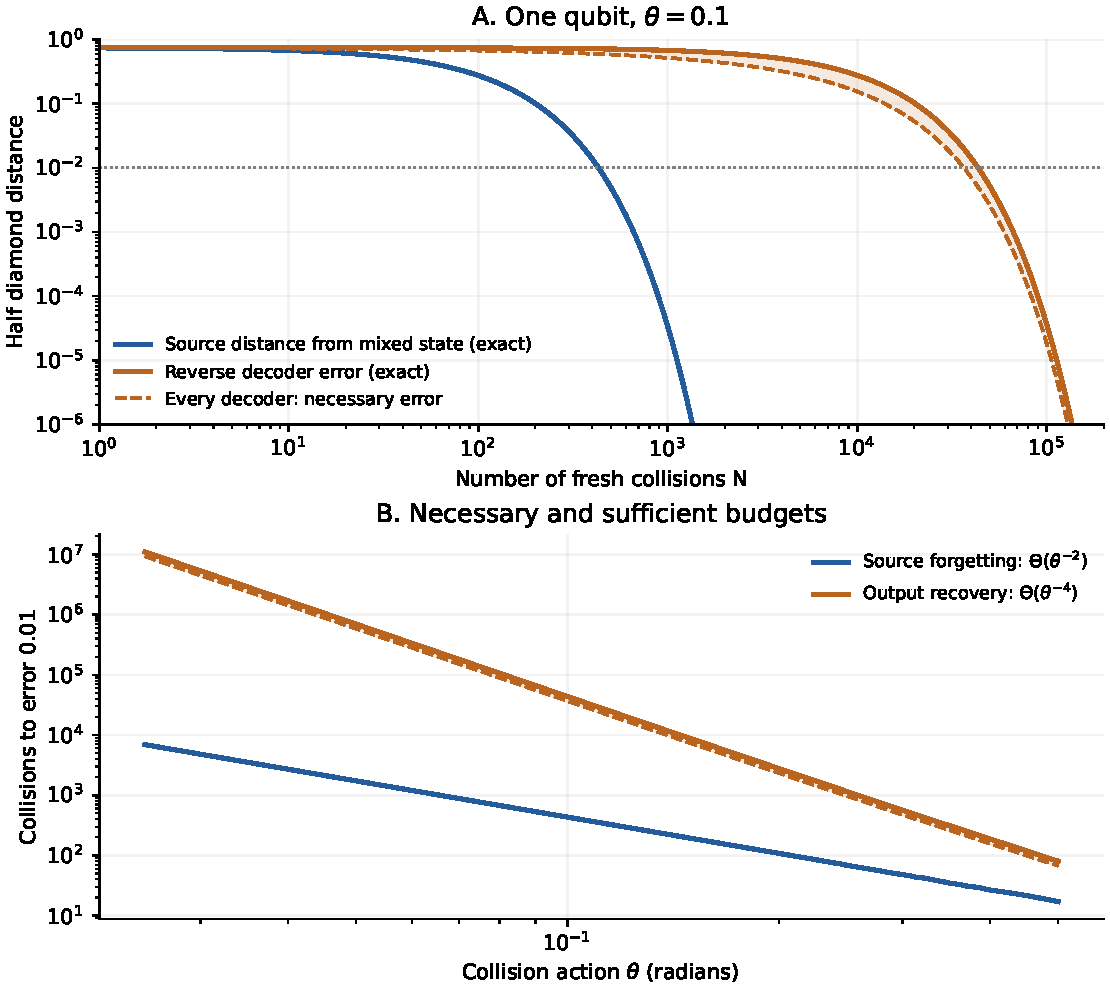
\includegraphics[width=\linewidth]{figures/acquisition_clocks.pdf}
 \caption{The two clocks, evaluated from exact formulas. Panel A: for one qubit
 and \(\theta=0.1\), source-to-replacer distance \eqref{eq:forgetting},
 explicit recovery error \(3r_N/4\), and the lower bound
 \(3(1-\sqrt{1-r_N})/4\) for every decoder. Panel B: necessary and sufficient
 collision counts to reach half-diamond error \(0.01\).
 These curves are formula evaluations, not simulations of the displayed
 many-register systems.}
 \label{fig:clocks}
\end{figure}

\subsection{An exact source semigroup does not fix the output clock}
Set the source-only rotations to identity. Choose collision duration
\(\Delta\) and rate \(\gamma>0\) by
\begin{equation}
 \cos^2\theta=e^{-\gamma\Delta}.
 \label{eq:clockmatching}
\end{equation}
Here \(T=N\Delta\) is the ideal source collision clock, the sum of encounter
durations. Additional routing, settling, and decoding time is charged in
Section~\ref{sec:physical}; it is not included in this ideal clock.
At \emph{every} grid time \(T=N\Delta\), the source channel is exactly
depolarizing with visibility \(e^{-\gamma T}\). The bath residual is instead
\begin{equation}
 r_N=\left[1-(1-e^{-\gamma\Delta})^2\right]^{T/\Delta},
 \qquad \alpha_N=\gamma^2T\Delta+O(\Delta^2)
 \label{eq:markov}
\end{equation}
at fixed \(\gamma,T\). The exact projection recursion gives
\begin{equation}
 d_\diamond(\Ccal_N,\Rcal_{I_E/e})
   \le\min\{1,\tfrac12\sqrt{(d^2-1)\alpha_N}\}.
 \label{eq:exact-output-bound}
\end{equation}
Use \eqref{eq:reference-bound} with exact transfer \(\sin^4\theta_j\)
instead of \(4a_j^4\). The entire bath channel, including every
multiregister correlation, approaches a replacer as \(\Delta\to0\) at fixed
\(T\), while the source has a nontrivial relaxation law.

This is already exact at a coarse time \(h\). Compare \(M\) fresh weak
collisions with \(\cos^2\theta_M=e^{-\gamma h/M}\), against one collision
with \(\cos^2\theta_1=e^{-\gamma h}\). Their source channels at \(h\) are
identical. The weak protocol has \(\alpha_M\sim\gamma^2h^2/M\) and approaches
an input-independent bath. The single collision has
\(\alpha_1=(1-e^{-\gamma h})^2\) and receiver error
\(c_d[1-(1-e^{-\gamma h})^2]\), small for large \(\gamma h\).
Repeating blocks preserves equal source channels at every coarse time.

\begin{figure}[!htbp]
 \centering
 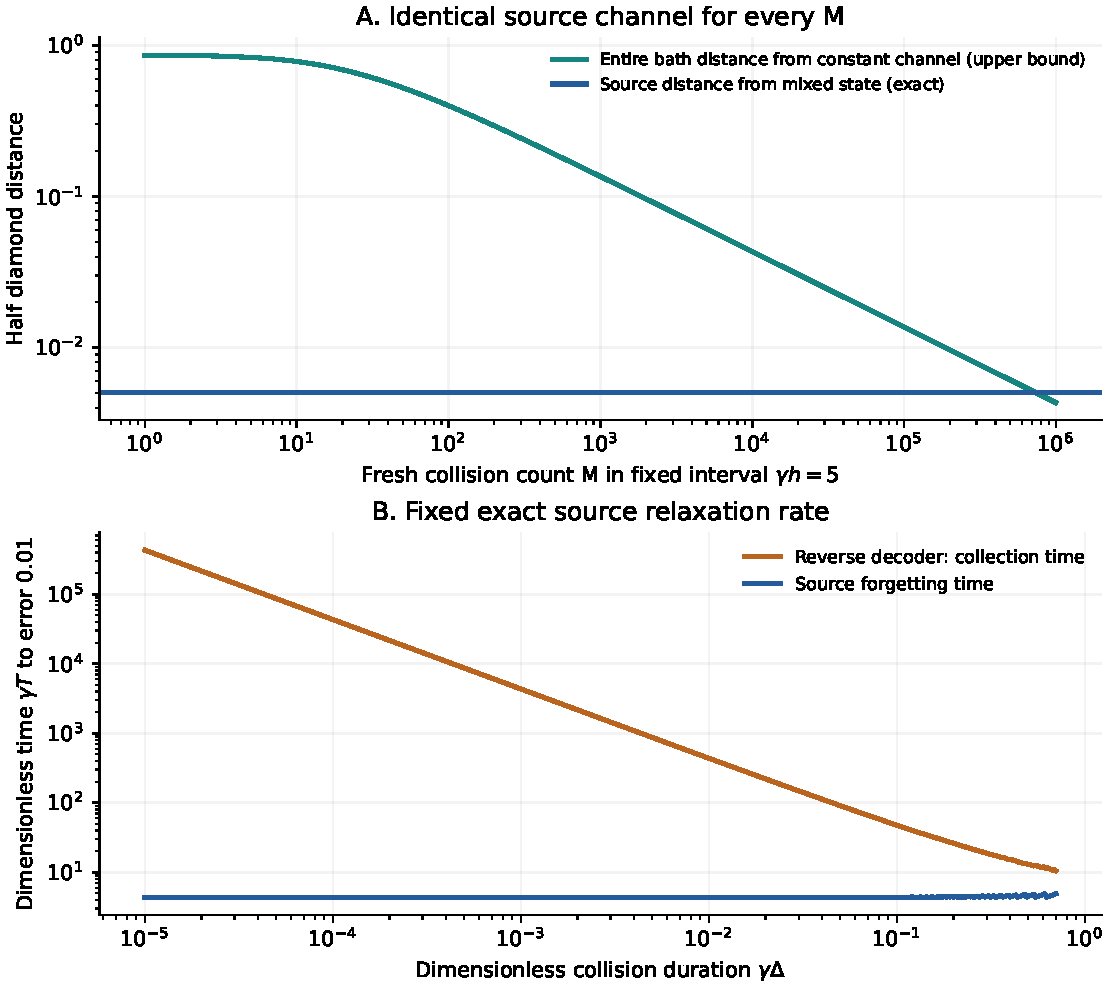
\includegraphics[width=\linewidth]{figures/same_source_dynamics.pdf}
 \caption{Output access is not determined by the source channel.
 Panel A: \(M\) fresh collisions over \(\gamma h=5\) have the same exact source
 channel for every \(M\), while the entire bath approaches a replacer.
 Panel B: fixing the exact grid-time relaxation rate \(\gamma\), source
 forgetting has bounded dimensionless time but native output collection time
 diverges as the collision interval decreases. All quantities use
 half-diamond error and exact formulas. Fixed-rate shrinking intervals
 require diverging coupling strength. Native times exclude the additional
 routing and decoder costs of the finite local implementation.}
 \label{fig:same-source}
\end{figure}

\subsection{Simultaneous limits and their physical price}
Both source and entire bath marginals can become input independent in one
family: take \(\Delta\to0\) and
\(T=\Delta\lceil\log[1/(\gamma\Delta)]/(\gamma\Delta)\rceil\).
Then \(\beta_N=O(\gamma\Delta)\) and
\(\alpha_N=O(\gamma\Delta\log[1/(\gamma\Delta)])\).
At every finite size, the joint source-plus-bath inverse restores the input
exactly. Input dependence can remain in their joint correlations when
neither marginal reveals it. No-hiding concerns the complete pure dilation,
including the initially inaccessible purifiers \cite{BraunsteinPati};
there is no contradiction.

Holding \(\gamma\) fixed requires \(\theta\sim\sqrt{\gamma\Delta}\).
A square exchange pulse has strength
\(\theta/\Delta\sim\sqrt{\gamma/\Delta}\), which diverges. The acquisition
exponent per physical time is asymptotically \(\gamma^2\Delta\), so collection
requires order \(\log(1/\eps)/(\gamma^2\Delta)\) time.
At fixed bounded strength \(J\), with \(\theta=J\Delta\), source forgetting
takes order \(1/(J^2\Delta)\) and recovery order \(1/(J^4\Delta^3)\),
up to accuracy logarithms. Repeated-interaction limits and their Hamiltonian
scalings are established \cite{AttalPautrat}; the limit does not supply
unlimited coupling, switching, or memory.

\section{Finite construction and uncertainty budget}
\label{sec:physical}
\subsection{Finite exchange hardware and a routing schedule}
This qubit construction is conditional on stated control and error
capabilities. It uses \(N+2\) cells: source, \(N\) memory cells, and a distinct
mixed dummy. Initialize and calibrate before loading the unknown payload;
otherwise charge its extra waiting time. The nearest-neighbor primitive is
\[
 U(\phi)=e^{-i\phi W},\quad H(t)=\hbar g(t)W,\quad
 \phi=\int g(t)\dd t,\quad |g|\le J.
\]
For spins \(W=(I+XX+YY+ZZ)/2\), isotropic exchange up to a scalar.
An \(XY\) interaction alone is not this primitive. Retain the scalar's
constant if the norm budget includes it. Known free evolution is tracked;
unknown drift is an error.

The source service supplies one encounter of maximum duration
\(\tau_{\rm enc}\) per fresh logical register, with \(|g|\le J_S\).
It therefore enforces \(a\le J_S\tau_{\rm enc}\); the encounter cannot be
paused, extended, or repeated on the same token. This timing/reach contract
is a supplied source-access restriction, not a consequence of bounded
strength alone. If duration can reach \(\pi/(2J_S)\), a single source SWAP
exports the input and is the stronger operation. Receiver routing SWAPs
do not supply that source access.
Signed receiver exchange implements the inverse in time \(\theta/J_M\).
Positive-only exchange uses angle \(\pi-\theta\), since
\(U(\pi-\theta)=-U(\theta)^\dagger\), at the longer duration.

Place \(S\) at \((-1,0)\), the memory at
\((0,0),(1,0),\ldots,(N-1,0)\), and the dummy at \((0,1)\).
The junction has \(N+2\) vertices, \(N+1\) edges, and maximum degree three.
In capture round \(j\), a fresh logical register at cell 1 meets the source.
Bubble the emitted token right through the remaining fresh tokens with
\(N-j\) full SWAPs, stopping before old outputs. Full SWAPs permute factors,
so future inputs stay fresh. The final order is \(E_N,\ldots,E_1\).
Close the source edge permanently.

Inverse-collide the side-branch dummy with \(E_N\), then SWAP the dummy
token into cell 1. Inverse-collide with \(E_{N-1}\), move right, and
continue; omit movement after the last inverse collision. This implements
the reverse logical circuit without source access, measurements, or
postselection. All correlations survive until coherent use.
The exact routing and total two-qubit gate counts are
\begin{align}
 R_c&=N(N-1)/2,&R_d&=N-1,\\
 R&=(N-1)(N+2)/2,&G&=2N+R=(N^2+5N-2)/2.
 \label{eq:gate-counts}
\end{align}
A strict line \(S,E_1,\ldots,E_N,D\) first moves the dummy left through
the outputs, adding \(N\) routing SWAPs.
Let \(\tau_c=\theta/J_S\), \(\tau_d=\theta/J_M\), and
\(\tau_w=\pi/(2J_M)\), replacing \(\tau_d\) by \((\pi-\theta)/J_M\)
for positive-only receiver exchange. If \(\tau_{\rm ctl}\) bounds
switching, addressing, and settling per gate, the serial schedule has
\begin{align}
 T_c&=N\tau_c+R_c\tau_w+(N+R_c)\tau_{\rm ctl},\\
 T_d&=N\tau_d+R_d\tau_w+(N+R_d)\tau_{\rm ctl},\\
 T_{\rm op}&=T_c+T_d,\qquad V_M\le(N+1)T_{\rm op}.
 \label{eq:times}
\end{align}
Here \(T_c\) is source exposure and \(V_M\) bounds coherent memory
space-time in qubit-time units. At fixed strengths and latency this
layout takes \(O(N^2)\) time and \(O(N^3)\) memory space-time. Optimal
native collision count does not imply optimal wall time for this layout.
For weak \(\theta\), the resulting powers can be \(\theta^{-8}\) for time
and \(\theta^{-12}\) for memory space-time, with accuracy logarithms.

\subsection{A joint preparation bound and an exact finite factory}
Suppose the actual \(L\) initial qubits are independent states \(\tau_j\).
Put \(x_j=2\Tr(\tau_j^2)-1\). Their global preparation error obeys
\begin{equation}
 \frac12\norm{\bigotimes_j\tau_j-(I/2)^{\otimes L}}_1
 \le\frac12\sqrt{\prod_j(1+x_j)-1}.
 \label{eq:prep-bound}
\end{equation}
For \(Q=2^L\), Cauchy--Schwarz gives
\(\norm{\rho-I/Q}_1^2\le Q\Tr\rho^2-1\), and product purity factors.
Replacing an input-independent environment changes the resulting channel
by at most this trace distance, uniformly in the payload/reference.
Apply it once to the whole process, not repeatedly to correlated outputs.

For Bloch vectors of norm at most \(\beta\), including the dummy so that
\(L=N+1\), a sufficient condition for preparation error at most \(\eps_p\) is
\begin{equation}
 \beta^2\le\frac{\log(1+4\eps_p^2)}{L}.
 \label{eq:prep-tolerance}
\end{equation}
This requires \(\beta=O(\eps_p/\sqrt N)\). Local tracial marginals do not
certify the product assumption. Correlated preparation needs a global bound
or a sum of composable preparation-channel errors.

Exact tracial preparation need not mean literal infinite-temperature
equilibration. Independent uniform Pauli randomization with inaccessible
keys satisfies
\[
 \frac14\sum_{P\in\{I,X,Y,Z\}}
   (P\otimes I)\rho(P^\dagger\otimes I)
       =I/2\otimes\Tr_{\rm qubit}\rho.
\]
It removes initial correlations in the ideal gate model, costing two
uniform classical bits and at most two Pauli pulses per cell, plus key
generation and disposal. Every copy of the operating keys must be unavailable
to receiver and future source controller. An accessible but unused key
still supplies a nontracial conditional bath and changes the interface.
Approximate twirls on correlated raw cells require composable channel-error
bounds; they do not automatically justify the product formula.
\subsection{Composable physical error and isolation}
Let \(\eta_g\) bound each gate's half-diamond error uniformly with arbitrary
entangled spectators. Let \(\kappa_S\) bound half the diamond norm of the
unwanted source noise generator during collection. Let \(\kappa_M\) give a
per-qubit bound whose sum controls the global memory generator.
Direct composable interval errors can replace this generator model.
Correlated noise needs a global bound; separate coherence times alone do
not establish it.

Source isolation is a distinct requirement. Residual coupling to retained
outputs supplies coherent feedback, outside the ideal interface.
During every closed interval, including decoder operation while the source
remains nearby, charge
\begin{equation}
 \eps_{\rm off}:=
 \int_{\rm closed}\norm{H_{\rm off}(t)}_\infty\dd t/\hbar
 \label{eq:isolation}
\end{equation}
as a sufficient perturbation bound, or use a directly certified channel
bound. It cannot be replaced by a source-only storage estimate.

Duhamel expansion, telescoping, and CPTP contraction give
\begin{align}
 d_\diamond(\widetilde{\Dcal\Ccal},\id)
 \le{}&\tfrac34(1-\sin^4\theta)^N+\eps_{\rm init}
       +\sum_g\eta_g+\kappa_ST_c+\kappa_MV_M \notag\\
     &+\eps_{\rm off}+\eps_{\rm other}.              \label{eq:physical-error}
\end{align}
The last term covers otherwise uncounted leakage, drift, delay, key leakage,
or cross-talk. Avoid double-counting errors already included elsewhere.
This bound is reference uniform and assumes no independence of the emitted
outputs.

One finite sufficient budget allocates \(\eps/2\) to the intrinsic first
term and \(\eps/10\) each to preparation, gates, source storage, memory
storage, and isolation, with no uncounted remaining errors. Thus take
\begin{align}
 N&\ge\frac{\log[(3/4)/(\eps/2)]}{-\log(1-\sin^4\theta)},&
 \eta_g&\le\frac{\eps}{10G},\\
 \beta^2&\le\frac{\log(1+\eps^2/25)}{N+1},&
 \kappa_S&\le\frac{\eps}{10T_c},\\
 \kappa_M&\le\frac{\eps}{10V_M},&
 \eps_{\rm off}&\le\frac{\eps}{10}.                  \label{eq:budget}
\end{align}
These conditions are conservative and sufficient. A protected logical
implementation must add its encoding, factories, ancillas, gates, latency,
and certified errors; none is supplied for free.

If actual emission is within \(\nu\) of ideal emission in half-diamond
distance, its optimal recovery error is at least the ideal lower bound
minus \(\nu\). Its distance from its \emph{own} replacer baseline is at most
the ideal output bound plus \(2\nu\). A fixed preparation bias cannot be
discarded as \(N\) grows.
For \(m\) independent physical modules, use the global intrinsic term in
\eqref{eq:module-exact}, \(m(N+1)\) initialized cells, and the actual summed
gate and space-time error budgets. Parallel operation reduces wall time
but does not remove these summed physical error exposures.
\subsection{Finite qualification and its exposure cost}
Preparation qualification assumes stationary, reproducible, independent
factories and trusted Pauli readout. For each of \(L=N+1\) cell types,
measure \(X,Y,Z\) on disposable preparations. If the empirical Bloch norm
is at most \(\beta/2\) and each mean has error at most
\(h\le\beta/(2\sqrt3)\), the true norm is at most \(\beta\).
Hoeffding's inequality and a union bound give
\begin{equation}
 M_p\ge24\beta^{-2}\log(6L/\alpha_p)
 \label{eq:prep-shots}
\end{equation}
trials per axis and cell, or \(3LM_p\) total. At
\(\beta=\Theta(\eps_p/\sqrt N)\), this is
\(O(N^2\eps_p^{-2}\log(N/\alpha_p))\).
Known preparation/readout systematics must fit inside the mean tolerance.
These data do not certify independence, hidden-side-channel absence, or
future stability. Calibration consumes no payload copies.

If exchange \emph{form} is independently promised, prepare \(\ket{01}\),
apply the pulse, and measure \(Z\otimes I\) and \(X\otimes Y\) separately.
Their means are \(\cos(2\phi)\) and \(\sin(2\phi)\), identifying angle
modulo the irrelevant global phase period \(\pi\).
Angle precision \(h_\phi\) costs
\(O(h_\phi^{-2}\log(K/\alpha_g))\) trials, also near zero because the
second signal is linear there. Angle error \(\delta\phi\) gives at most
\(|\delta\phi|\) half-diamond gate error. Inverse control needs qualification
too. Scalar tests do not certify generic exchange form or absence of
leakage and cross-talk.

A general certificate assumes a closed, stationary, context-independent
two-qubit CPTP gate and trusted preparation/readout.
For each distinct configuration, prepare its normalized Choi state using
two input/reference Bell pairs, act on the two inputs, and measure all
\(L_P=4^4-1=255\) nonidentity four-qubit Paulis separately.
Each trial uses four qubits, two trusted Bell pairs, one tested gate, and
four Pauli readouts. These references are paid calibration resources,
not operating bath purifiers.

For input dimension \(q=4\), let \(\widehat r_P\) estimate
\(r_P=\Tr(JP)\) with statistical width \(h\) and known systematic width
\(s_P\). A direct certificate is
\begin{equation}
 d_\diamond(\mathcal E,\mathcal U)
 \le\frac q2\sqrt{\sum_{P\ne I}
    \bigl(|\widehat r_P-r_P^{\rm ideal}|+h+s_P\bigr)^2}.
 \label{eq:gate-certificate}
\end{equation}
Pauli orthogonality and trace/Hilbert--Schmidt comparison imply
\(\norm{J_{\mathcal E}-J_{\mathcal U}}_1
\le\sqrt{\sum_P(\delta r_P)^2}\).
Together with
\(\norm{\mathcal E-\mathcal U}_\diamond
\le q\norm{J_{\mathcal E}-J_{\mathcal U}}_1\)
this proves the certificate without requiring a physical reconstructed map.

With \(K\) configurations, simultaneous statistical width \(h\) requires
\begin{equation}
 M_g\ge2h^{-2}\log(2L_PK/\alpha_g)
 \label{eq:gate-shots}
\end{equation}
trials per Pauli and configuration. Take
\(h=O(\eta/(q\sqrt{L_P}))\) and control systematics similarly.
Here \(K\le2N+1\): one source pulse, at most \(N\) receiver inverse locations,
and \(N\) routing locations. With \(G=O(N^2)\) and
\(\eta=\Theta(\eps/G)\), the sufficient general qualification bill is
\begin{equation}
 KL_PM_g=O\!\left(N^5\eps^{-2}\log(N/\alpha_g)\right).
 \label{eq:qualification-cost}
\end{equation}
This is conservative; shared-parameter savings need independent
justification. Low collision count does not hide the qualification cost.

Each gate trial takes actual Bell-preparation, pulse, readout, reset, and
control time, multiplied by the displayed trial count and settings.
Factory qualification takes \(3LM_p\) actual preparation/readout/reset
cycles. The ideal twirling factory additionally costs up to \(2L\) Pauli
pulses, \(2L\) uniform random bits, and their inaccessible disposal.
Trusted references and sensors cannot be obtained for free from the same
unqualified devices. Source-edge tests precede payload loading or use a
justified equivalent replica.
On the joint confidence event, probability at least
\(1-\alpha_p-\alpha_g\), the physical budget is reference uniform.
Finite data qualify approximation under the stated model; they do not prove
exact zero error, absence of all hidden interactions, or arbitrary future
stability.

\paragraph{Global qualification for \(m\) modules.}
Without a shared-parameter reduction, the register construction has
\[
 G_{\rm tot}=m(N^2+5N-2)/2,\quad
 K_{\rm tot}\le m(2N+1),\quad L_{\rm tot}=m(N+1).
\]
Allocating a global gate error \(\eps_g\) sets per-gate tolerance of order
\(\eps_g/G_{\rm tot}\). Thus sufficient general gate qualification is
\[
 O\!\left(m^3N^5\eps_g^{-2}\log(mN/\alpha_g)\right)
\]
trials. A global product-preparation budget \(\eps_p\) gives sufficient
factory qualification
\[
 O\!\left(m^2N^2\eps_p^{-2}\log(mN/\alpha_p)\right).
\]
For parallel identical modules the elapsed operation time remains
\(T_{\rm op}\), while memory space-time is at most
\(m(N+1)T_{\rm op}\). Serial execution also charges every initially present
payload's waiting time before its own module begins. These explicit
conservative bills may be reduced by justified common-parameter hardware,
parallel test equipment, or improved certificates; none is silently assumed.

\section{Executed evidence and resource evaluations}
\label{sec:evidence}
The accompanying program constructs the actual finite channels and inverse
receiver. It does not replace proof by testing.
In 48 dense qubit cases, \(N=1,\ldots,6\), four base angles, and with
noncommuting known source rotations in half the cases, the program retains
the full \(2^N\)-dimensional bath. It computes the operator Gram matrix and
applies the inverse circuit to an independent mixed dummy after discarding
the real source. The maximum Gram discrepancy is
\(9.9921\times10^{-16}\), and the maximum decoder-map discrepancy is
\(1.1103\times10^{-15}\).

Five additional dense cases use \(d=3,4\), \(N\le3\), source rotations, and
random mixed entangled input/reference states with reference dimension
\(d+1\). They evolve the joint state, trace out the actual source, append an
independent dummy, and reverse the stored-output circuit. The largest
entrywise discrepancy from \eqref{eq:exact-recovered} tensored with the
reference identity is \(5.563\times10^{-17}\).

Eighty generic two-qubit Hamiltonians test the single-round amplitude
estimate \(2a^2\); the largest observed ratio to that bound is \(0.397592\).
Twelve selected feedback chains measure emitted qubits, keep their complete
records, and choose subsequent interactions from preceding outcomes. Their
Bell-input trace distances satisfy the general bound. These are
floating-point diagnostics of the implementation and conventions. They
do not establish an all-Hamiltonian theorem or the full diamond norm by
sampling. The unrestricted-decoder converse is analytic; no optimization of
optimal decoders or hardware experiment was performed.

\begin{table}[!htbp]
 \centering\small
 \begin{tabular}{@{}rrrrrr@{}}
 \toprule
 Modules & \(\theta\) & \shortstack{Source\\forgetting} &
 \shortstack{Every decoder\\necessary \(N\)} &
 \shortstack{Reverse decoder\\sufficient \(N\)} &
 \shortstack{Stored output\\qubits}\\
 \midrule
 1 & 0.05 & 1,727 & 581,933 & 691,949 & 691,949\\
 1 & 0.10 & 432   & 36,552  & 43,462  & 43,462\\
 1 & 0.20 & 108   & 2,329   & 2,770   & 2,770\\
 1 & 0.40 & 27    & 157     & 186     & 186\\
 1,000 & 0.10 & --- & 105,970 & 112,948 & 112,948,000\\
 \bottomrule
 \end{tabular}
 \caption{Qubit formula evaluations for target half-diamond error \(0.01\).
 Recovery counts \(N\) are per module; the last row targets the entire
 1,000-qubit register and permits collective final decoding. Source forgetting
 targets a single source's distance from its replacer, so that column is
 omitted for the joint-register row. Single-module converse counts use the
 sharper centered bound \eqref{eq:exact-sandwich}. These are not simulations
 with the displayed numbers of bath qubits. Routing, precision, and memory
 costs are additional.}
 \label{tab:counts}
\end{table}

The table and both figures evaluate proved formulas. For example,
\(\theta=0.1\) erases a source qubit to error \(0.01\) after 432 collisions,
but every bath-only decoder needs at least 36,552, while the explicit receiver
uses 43,462. An earlier coarse bound \(c_dr_N/2\) gives the valid but weaker
36,485 count. The tighter value in Table~\ref{tab:counts} uses
\(c_d(1-\sqrt{1-r_N})\).
For 1,000 independent modules at this angle, the explicit construction
retains 112,948,000 qubits before accounting for protection overhead. This
large cost is part of the result's practical interpretation.

These counts spend the entire \(0.01\) target on the ideal intrinsic error.
Allocating only \(\eps/2\) to that error in \eqref{eq:budget} increases \(N\)
before the physical preparation, gate, isolation, and storage costs are added.

The code, machine-readable records, exact resource formulas, and independent
proof/selection notes accompany this manuscript. Large-resource examples are
not claimed to have been physically executed, classically state-vector
simulated, or supported by an implemented fault-tolerant memory.

\section{Comparison with existing operations and accepted results}
\label{sec:prior}
\paragraph{Quantum homogenization.}
Ziman and collaborators introduced sequential partial SWAP, source
homogenization, correlation analysis, and a \emph{quantum safe} inverse
\cite{Ziman}. Their Section VII.B requires all \(N+1\) particles, identifies
the original source, and reverses the interactions. The present receiver
receives only the \(N\) emitted particles, substitutes an independent mixed
dummy, and pays the exact residual \(r_N\). The difference is physical access,
not a new partial-SWAP gate or a new observation that correlations matter.

Yosifov and collaborators study homogenizer circuits and reservoir
correctability using generalized B\'eny--Oreshkov conditions and a stipulated
approximately forgetful complementary channel \cite{Yosifov}.
Their reviewed Section IV does not supply the finite tracial output-only
\(\sin^4\theta\) clock or the adaptive action bound here. We do not refute
their conditional protection claim or equate their complement with the
unavailable purifiers of our physical model.

\paragraph{Transpose recovery and physical inversion.}
Petz recovery, Barnum--Knill near-optimality, and Renes's sharper inequality
are credited explicitly \cite{BarnumKnill,Renes}. Aw and collaborators give
product preservation as a sufficient condition for physical inverse-unitary
Petz implementation; Song and collaborators develop exact, approximate, and
collisional implementation conditions \cite{Aw,Song}.
The mixed-dummy inverse is an instance of that principle. Its generic
existence is not our novelty claim. The calculation those principles alone
do not provide is the acquired bath channel's complete information energy,
including classical feedback, and its exact finite acquisition clock.
Here the known reverse circuit also exposes its execution cost.

\paragraph{No-hiding, mixed dilations, and continuum limits.}
No-hiding refers to the complete pure dilation \cite{BraunsteinPati}.
The physical mixed bath can be a strict part of that complement.
Repeated-interaction limits have established mathematical machinery
\cite{AttalPautrat}. The present bound distinguishes the actual mixed output
from a purified noise representation and charges the strength needed to
keep source relaxation fixed.
Violaris and Marletto study reservoir deterioration when homogenizers are
reused for cyclic erasure \cite{Violaris}. That differs from recovering one
input from all first-use outputs after source disposal; no conclusion about
the economics of cyclic erasure is claimed.

\paragraph{Accepted Astra premises and nearby results.}
Corpus comparisons use revision
\texttt{324acb589443002bf8d529cc15e160129c5e36d2}
\cite{AstraMarkov,AstraExtreme,AstraCollector}.
N1729 already gives a mixed classical-selector realization of a
random-unitary source channel with input-independent emitted selector.
It separately obtains a quartic finite-clock law for a \emph{pure}-bath,
two-collision driven-dephasing communication protocol. Neither
mixed-implementation ambiguity nor the occurrence of a fourth power alone
is a new consequence here.

N1733 proves that an extreme source channel's whole outgoing mixed bath is
isometrically equivalent to its minimal complement tensored with the initial
mixed bath, under explicit rank/access constraints. Its full-rank finite
bath obstruction rules out a nonunitary extreme same-dimension source.
The depolarizing source in the present regime is nonextreme; that positive
result does not supply our receiver with a missing purifier.

The latest P1 collector supplies calibrated pure coherent ports for a
many-body acquisition construction. Those are actual resources.
The tracial once-through interface here does not possess them. Our result
gives a quantitative boundary and attainable finite scale for a different
interface, without altering the pure-port construction's conditions.

\paragraph{The increment and its limit.}
The local cancellation \eqref{eq:first-order-zero} becomes an all-output law
through a contracting weighted norm and orthogonality of new and previously
exported contributions. It survives receiver instruments and pathwise
classical feedback. The partial-SWAP Gram identity supplies a matching
operation, and existing recovery inequalities convert it to optimality
bounds. Product-channel structure adds a joint-register cost, while equal
exact source dynamics show why a reduced generator cannot replace an
acquired-output specification.

The completed result certifies when a declared weak mixed-bath interface
cannot yet carry a recoverable arbitrary state, and gives a receiver attaining
the optimal scale with finite supplied resources. It does not identify an
unknown source, certify every hidden coupling from finite data, recover from
arbitrary thermal baths, or supply unlimited coherent memory. No exhaustive
priority claim or civilization-scale consequence is established.

\begin{thebibliography}{99}
\raggedright
\small
\setlength{\itemsep}{2pt}
\setlength{\parsep}{0pt}
\bibitem{Ziman}
M.~Ziman, P.~\v{S}telmachovi\v{c}, V.~Bu\v{z}ek, M.~Hillery,
V.~Scarani, and N.~Gisin,
\emph{Diluting quantum information: An analysis of information transfer in
system-reservoir interactions}, Physical Review A \textbf{65}, 042105 (2002).
\href{https://doi.org/10.1103/PhysRevA.65.042105}
{doi:10.1103/PhysRevA.65.042105}.
Preprint \emph{Quantum homogenization}:
\url{https://arxiv.org/abs/quant-ph/0110164}.

\bibitem{Yosifov}
A.~Yosifov, A.~Iyer, D.~Ebler, and V.~Vedral,
\emph{Quantum homogenization as a quantum steady-state protocol on noisy
intermediate-scale quantum hardware}, Physical Review A \textbf{109},
032624 (2024).
\href{https://doi.org/10.1103/PhysRevA.109.032624}
{doi:10.1103/PhysRevA.109.032624}.
\url{https://arxiv.org/abs/2412.14544}.

\bibitem{BarnumKnill}
H.~Barnum and E.~Knill,
\emph{Reversing quantum dynamics with near-optimal quantum and classical
fidelity}, Journal of Mathematical Physics \textbf{43}, 2097--2106 (2002).
\href{https://doi.org/10.1063/1.1459754}{doi:10.1063/1.1459754}.
\url{https://arxiv.org/abs/quant-ph/0004088}.
The current arXiv version includes a corrected proof.

\bibitem{Renes}
J.~M.~Renes,
\emph{Better bounds on optimal measurement and entanglement recovery, with
applications to uncertainty and monogamy relations}, Physical Review A
\textbf{96}, 042328 (2017), Eq.~(13).
\href{https://doi.org/10.1103/PhysRevA.96.042328}
{doi:10.1103/PhysRevA.96.042328}.
\url{https://arxiv.org/abs/1707.01114}.

\bibitem{Aw}
C.~C.~Aw, L.~H.~Zaw, M.~Balanz\'o-Juand\'o, and V.~Scarani,
\emph{Role of Dilations in Reversing Physical Processes: Tabletop
Reversibility and Generalized Thermal Operations}, PRX Quantum \textbf{5},
010332 (2024), Theorem~3.
\href{https://doi.org/10.1103/PRXQuantum.5.010332}
{doi:10.1103/PRXQuantum.5.010332}.
\url{https://arxiv.org/abs/2308.13909}.

\bibitem{Song}
M.~Song, H.~Kwon, and V.~Scarani,
\emph{Exact and approximate conditions of tabletop reversibility: when is
Petz recovery cost-free?}, Quantum Science and Technology \textbf{11},
045057 (2026).
\href{https://doi.org/10.1088/2058-9565/aea92d}
{doi:10.1088/2058-9565/aea92d}.
\url{https://arxiv.org/abs/2510.26895}.

\bibitem{BraunsteinPati}
S.~L.~Braunstein and A.~K.~Pati,
\emph{Quantum information cannot be completely hidden in correlations:
Implications for the black-hole information paradox},
Physical Review Letters \textbf{98}, 080502 (2007).
\href{https://doi.org/10.1103/PhysRevLett.98.080502}
{doi:10.1103/PhysRevLett.98.080502}.
\url{https://arxiv.org/abs/gr-qc/0603046}.

\bibitem{AttalPautrat}
S.~Attal and Y.~Pautrat,
\emph{From repeated to continuous quantum interactions},
Annales Henri Poincar\'e \textbf{7}, 59--104 (2006).
\href{https://doi.org/10.1007/s00023-005-0242-8}
{doi:10.1007/s00023-005-0242-8}.
\url{https://arxiv.org/abs/math-ph/0311002}.

\bibitem{Violaris}
M.~Violaris and C.~Marletto,
\emph{Irreversibility beyond Landauer's principle: is it possible to perform
erasure using the quantum homogenizer?},
New Journal of Physics \textbf{24}, 113030 (2022).
\href{https://doi.org/10.1088/1367-2630/ac9e13}
{doi:10.1088/1367-2630/ac9e13}.

\bibitem{AstraMarkov}
Astra Research, \emph{Markov bath communication onset}, N1729 and governing
source \texttt{P1\_MARKOV\_BATH\_COMPLETE\_RETURN.txt}.
\href{https://github.com/harjassand/astra-research-knowledge/blob/324acb589443002bf8d529cc15e160129c5e36d2/research/2026-11-04-markov-bath-communication-onset/source/P1_MARKOV_BATH_COMPLETE_RETURN.txt}
{Pinned governing source}, revision
\texttt{324acb589443002bf8d529cc15e160129c5e36d2}.

\bibitem{AstraExtreme}
Astra Research, \emph{Causal-state interface constructions}, N1733,
governing source \texttt{P1\_CAUSAL\_TRANSDUCTION\_COMPLETE\_RETURN.txt},
Section~6.
\href{https://github.com/harjassand/astra-research-knowledge/blob/324acb589443002bf8d529cc15e160129c5e36d2/research/2026-11-04-causal-state-interface-constructions/source/P1_CAUSAL_TRANSDUCTION_COMPLETE_RETURN.txt}
{Pinned governing source}, same revision.

\bibitem{AstraCollector}
Astra Research, \emph{Scalable many-body acquisition from pure coherent
ports}, P1 return package.
\href{https://github.com/harjassand/astra-research-knowledge/tree/324acb589443002bf8d529cc15e160129c5e36d2/research/returns/2026-11-05-p1-scalable-many-body-acquisition}
{Pinned source package}, same revision.
\end{thebibliography}
\end{document}
